%% 4. 「技術研究報告」
\documentclass[technicalreport]{ieicej}
%\usepackage[dvips]{graphicx}
\usepackage[dvipdfmx]{graphicx,xcolor}
\usepackage[T1]{fontenc}
\usepackage{lmodern}
\usepackage{textcomp}
\usepackage{latexsym}
%\usepackage[fleqn]{amsmath}
\usepackage{amssymb}
\usepackage{subfigure}

\jtitle{ LTE 環境における応答遅延特性の時系列モデリングによる分析}
\jsubtitle{}
\etitle{Analysis of delay characteristics of connection through LTE by time series analysis}
\esubtitle{}
\authorlist{%
 \authorentry[k-yamamt@ist.osaka-u.ac.jp]{山本 航平}{Kohei YAMAMOTO}{Osaka}
 \authorentry[wakamiya@ist.osaka-u.ac.jp]{若宮 直紀}{Naoki WAKAMIYA}{Osaka}
 \authorentry[ryo.nakano.xd@hitachi.com]{中野 亮}{Ryo NAKANO}{hitachi}
 \authorentry[ryosuke.fujiwara.mb@hitachi.com]{藤原 亮介}{Ryosuke FUJIWARA}{hitachi}
% \authorentry[メールアドレス]{和文著者名}{英文著者名}{所属ラベル}
}
\affiliate[Osaka]{大阪大学大学院情報科学研究科バイオ情報工学講座\\ 〒565-0871 大阪府吹田市山田丘 1-5}{Department of Bioinformatic engineering,Graduate school of Information Science and Technology,Osaka University\\ 1-5 Yamadaoka, suita-shi, Osaka, 565-0871, Japan}
\affiliate[hitachi]{株式会社日立製作所 研究開発グループ\\ 〒185-8601 東京都国分寺市東恋ヶ窪 1-280}{Research \& Development Group, Hitachi, Ltd.\\ 1-280 Higashikoigakubo, kokubunji-shi, Tokyo, 185-8601, Japan}
%\affiliate[所属ラベル]{和文勤務先\\ 連絡先住所}{英文勤務先\\ 英文連絡先住所}

\begin{document}
\begin{jabstract}
%和文あらまし
産業用モニタリングシステムにおける運用管理コストの低減のため,迅速な障害検知・予測,ならびに原因の特定と対処法の提示が求められている.その実現にむけて,無線機器からサーバまでのLTE回線を含む通信路について,異なる時間帯において応答遅延の計測を行った.本稿では,遅延の変動特性や,曜日や時間帯に依存した傾向の有無について,時系列モデルを用いたクラスタリングによって分析した結果を示す.
\end{jabstract}
\begin{jkeyword}
%和文キーワード
Long Term Evolution,応答遅延,時系列モデリング,異常検知
\end{jkeyword}
\begin{eabstract}
%英文アブストラクト
In order to reduce the costs of operation and management in industrial monitoring systems, it is necessary to detect or predict failures quickly, identify the cause, and present countermeasures. To achieve this, we measured response delays of connection from one wireless device to one server, includeing LTE, in different time zones.In this technical report, we show the results of analyzing the fluctuation characteristics of responce delay and the tendency depending on the day of week or time zone by clustering using a time series analysis.
\end{eabstract}
\begin{ekeyword}
%英文キーワード
Long Term Evolution,response delay,time series analysis,anomaly detection
\end{ekeyword}
\maketitle

\section{はじめに}
近年,IoT (Internet of Things) 技術の発展とともに産業用モニタリングシステム\cite{monitering}が普及している.
これは,工場などの産業施設に設置された機器から直接,あるいは配置したカメラやセンサーなどの IoT デバイスを通じて,機器の稼働状態に関する情報をリアルタイムで収集し,キャリア回線を通じてクラウドサーバに送信,さらにクラウドサーバでデータ処理を行い,運用管理担当者に提示するものである.
従来作業員が巡回し行っていた工場内の機器の点検業務を自動化できるため,人員コストの軽減,目視確認より生じる人的ミスの低減,リアルタイムなデータの利活用などの効果が期待できる.
一方で,長期間の運用のなかで機器に具備された IoT デバイスの故障,工場内ネットワークの通信の途絶,クラウドサーバへの通信の遅延などの障害は避けられない.
このような障害が発生した場合には工場内の機器の稼働状況を把握することが困難となり,工場の稼働停止や業務の遅れなどが引き起こされ大きな損失をもたらす可能性がある.

障害発生時には迅速な復旧作業が求められるが,障害はその原因や内容,規模よってさまざまである.
しかしながら,現状ではシステムから得られる情報を用いてこれらの障害を適切かつ迅速に区別することが困難であるため,障害発生時には運用管理担当者が直接現場に行き障害の原因や内容,規模を確認する必要があり,多大な運用管理コストが発生している.
そのため,モニタリングシステムによる運用管理コストの低減のためには,直接また間接的に取得できる情報にもとづいて,障害発生を迅速に検知また予測するとともに,障害の原因を特定し,加えてその対処法を示すことが求められている.

すでに我々の研究グループでは機器間で測定される受信電波強度の時間変化にもとづいて空間的な電波伝搬特性の変動を推定することにより工場内での無線通信の異常を検知する手法を提案している\cite{prev}.
そこで,本報告では工場内で機器稼働情報を収集する無線機器からクラウドサーバまでの通信路で発生する異常の検知にむけてさまざまな曜日,時間帯で応答遅延を計測し特性の分析を行う.
具体的には,キャリア回線として産業用モニタリングシステムに広く用いられている LTE(Long Term Evolution)回線を用いる.
LTE 回線に関する研究として,応答遅延時間を他の無線回線と比べて評価を行った研究\cite{lte1}\cite{lte2}や LTE 環境下での TCP パケットの振る舞いに関する調査\cite{tcp},LTE 環境の応答遅延において,人の混雑状況にかかわらず発生する低遅延帯の分布が部分正規分布に従うことを示唆した研究\cite{distribution}などが行われている.
しかし,LTE を利用したインターネットとの通信において発生する遅延などの異常を検知・予測するといった観点からの通信特性の多角的な分析は十分になされていない.
そこでまずは分析に用いる実測データの収集として,月曜日から日曜日の 3 時,7 時,12 時,17 時,20 時のそれぞれ 1 時間において私が在籍している研究室内に設置した無線端末から AWS サーバへ ping による応答遅延の計測を行った.
計測した応答遅延に,例えば曜日,時間帯に依存した傾向が認められれば,その傾向と対比することによって応答遅延の通常ではない振る舞い,すなわち異常を検知することができる.
そこで,時系列モデリングによる回帰で得られたパラメータやその主成分を用いてクラスタリングすることで計測データをグループ化し,共通する特徴を見いだす.

第 2 章では本報告で実施した計測実験の設定について述べる.
第 3 章では時系列モデルによる回帰について述べる.
第 4 章では回帰結果に用いたクラスタリングにもとづく分析について述べる.
第 5 章では全体のまとめと今後の課題について述べる.
\section{計測実験の設定}
本報告では図 \ref{exp} に示す構成で計測実験を行った.
モニタリングシステムにおける無線端末としては LTE モジュールとして Quectel 社製 EC21-J を搭載した Raspberry Pi を用いた.
また,LTE 回線としては IIJ モバイル社のサービスタイプ D 定額プランライト(いちねん プリペイド)を用いた.
IIJ モバイル社は他の通信事業者から通信回線を借り受け,サービスを提供している MVNO(Mobile Virtual Network Operator)であり,サービスタイプ D では NTT ドコモ社の回線を使用している.
月あたり通信量が 3GB を超過すると通信速度が 256kbps に制限されるが,本実験中には速度制限は課されなかった.

クラウドサーバとしては本計測を行うにあたり契約した一台の AWS サーバを用い,大阪大学敷地内の研究室に設置した Raspberry Pi から ping を用いて応答遅延を計測した.
自動的に計測データを取得できるよう,Raspberry Pi 上で動作する Raspbian において計測用のスクリプトを用いることで, 15 秒毎に時刻を取得し,続けて ping (パケットサイズ 60 バイト, ICMP ECHO メッセージ,パケット数 1 )を実行した.
計測時刻,ping の出力をログデータとして取り出し,分析を行った.
また,日時が応答遅延に与える影響を調べるため,様々な時間帯で計測を行った.
計測は 2/29(土)から 3/27(金)までの四週間に渡って行った.

\begin{figure}[tb]
\centering
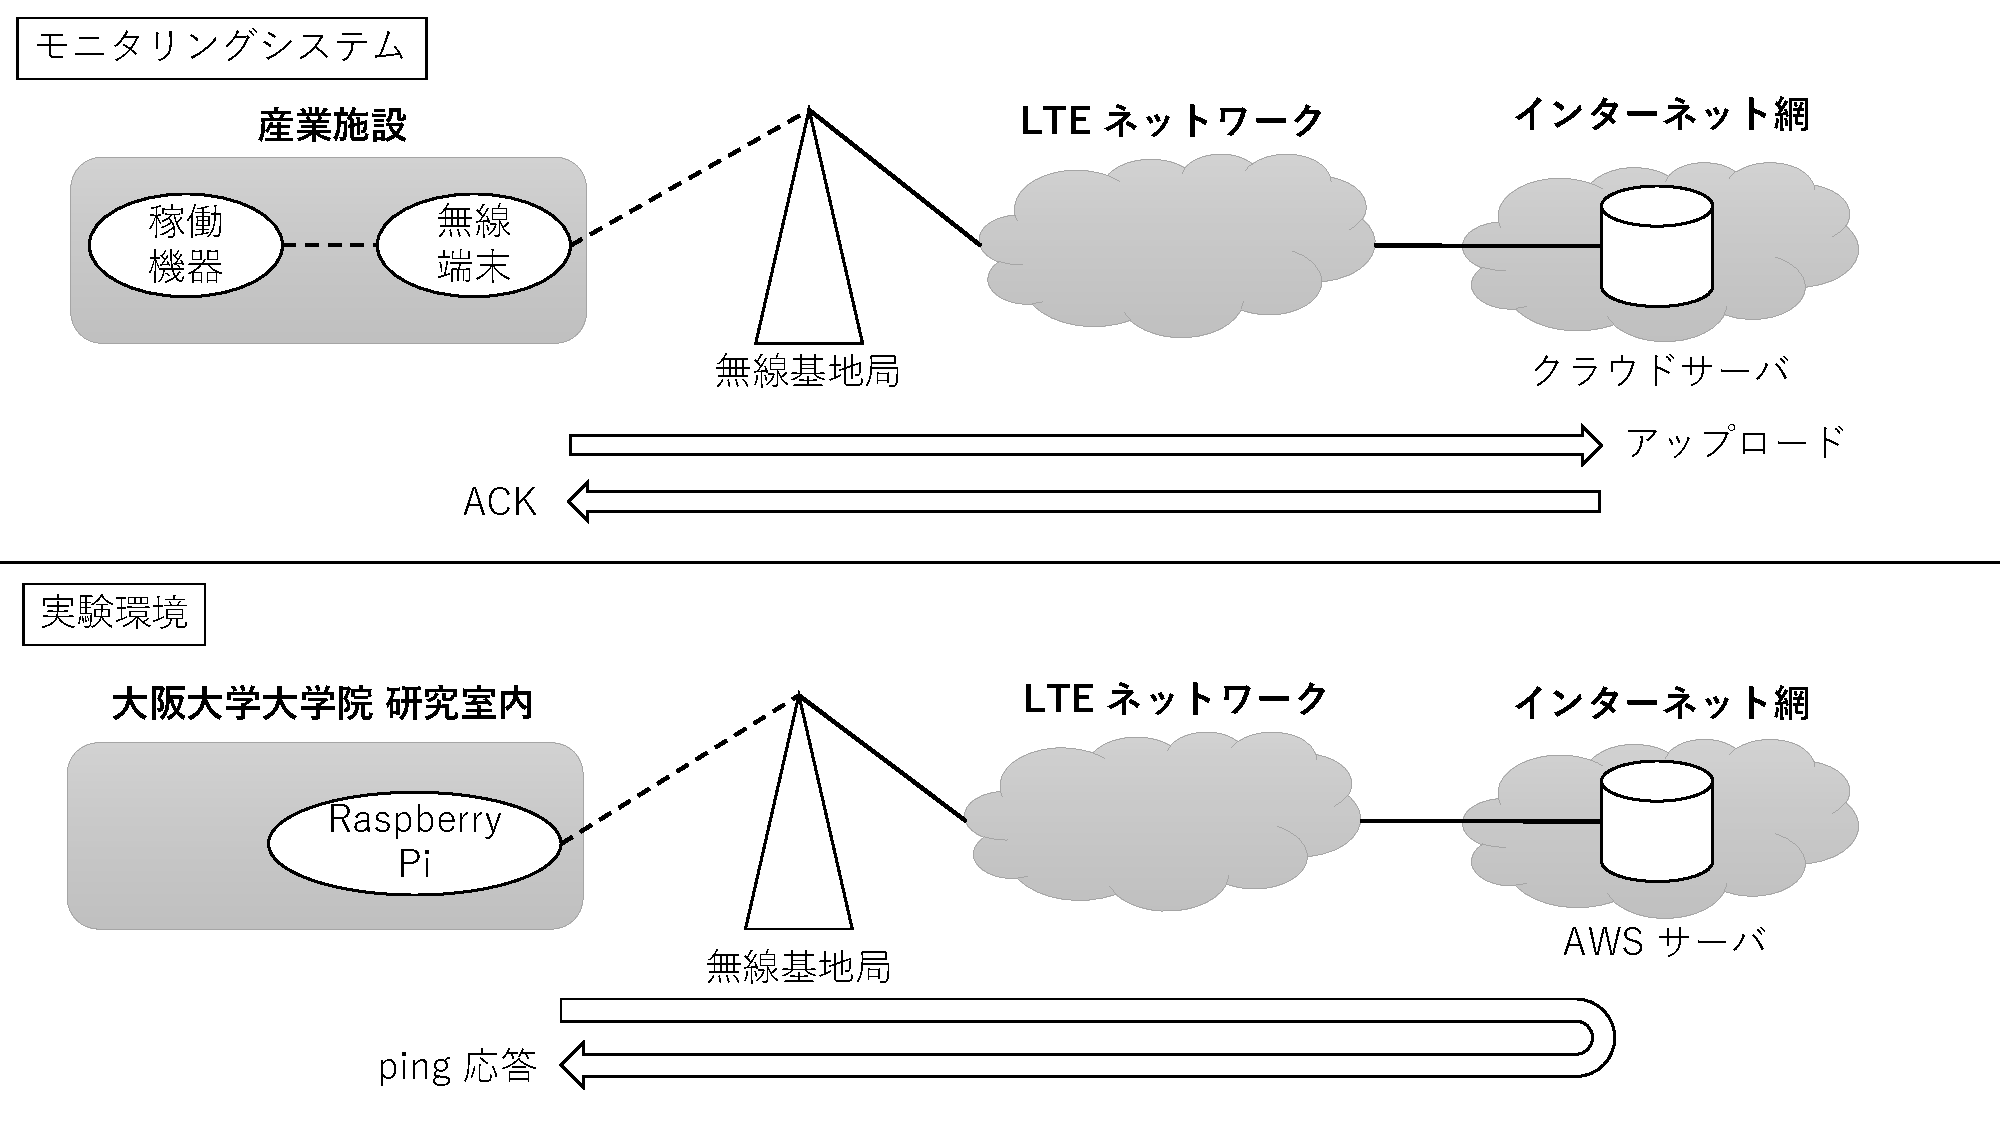
\includegraphics[width=7.5cm]{experiment.pdf}
\caption{モニタリングシステムと実験環境の対応図}
\label{exp}
\end{figure}

\section{時系列モデルによる回帰}
本報告では,時系列モデルとして式 (\ref{garch1}) と式 (\ref{garch2}) で表される ARMA-GARCH(Autoregressive Moving Average - Generalized Autoregressive Conditional Heteroscedasticity)モデル\cite{arma-garch}を用いる.
\begin{equation}
y_t = \sum_{i=1}^p a_i y_{t-i} + \sum_{i=1}^q b_i \varepsilon_{t-i} + c + \varepsilon_{t} 
\label{garch1}
\end{equation}
$$\varepsilon_t \sim N(0,h_t) \hspace{0.5cm} \rm{i.i.d}$$
\begin{equation}
\displaystyle h_{t} = \omega + \sum_{i=1}^{r}\alpha_i\varepsilon_{t-i}^2 + \sum_{i=1}^{s}\beta_ih_{t-i}
\label{garch2}
\end{equation}

時系列モデルによる回帰では,適切な次数 $p,q,r,s$ のもとで実測値 $y_t$ の時系列を最も精度良くモデル化できるパラメータ $a_i,b_i,c,\omega,\alpha_i,$および $\beta_i$ を算出する.
ここで,$y_t(1\leq t\leq N,N=240)$は1時間の計測実験のそれぞれにおける計測時刻順の実測値である.
また,$c$ は定数項,$\varepsilon_t$ は平均0,分散 $h_t$ の独立同一な正規分布に従うノイズ項である.
したがって,時刻 $t$ における実測値 $y_t$ は,過去の $p$ 時点前までの実測値と $q$ 時点前までのノイズ項のそれぞれの重み付き和と自身のノイズ項によって表される.
また,式 (\ref{garch2}) において,$\omega$ は定数項であり,時刻 $t$ におけるノイズ項が従う正規分布の分散 $h_t$ は,過去の $r$ 時点前までのノイズ項と $s$ 時点前までのノイズ項が従う正規分布の分散のそれぞれの重み付き和によって表される.

次数と呼ばれるパラメータ $(p,q,r,s)$ は対象とする時系列データに応じて適切に定める必要がある.
最適な次数は計測実験ごとに異なるが,クラスタリングによる分類,分析のために共通の次数を用いることとする.
次数 $0\leq p\leq2,0\leq q\leq 2,r=1$,および $0\leq s\leq 1$ のそれぞれの組み合わせに対してAIC(赤池情報量規準)\cite{aic1}\cite{aic2}を求めたところ,最大次数である $(p,q,r,s)=(2,2,1,1)$ が最適な計測区間が存在することから,これを共通の次数として用いることとした.
本報告では,式 (\ref{garch1}) に関与する $p,q$ の探索範囲の上限は回帰モデルが複雑になりすぎないようにともに 2 までとし,式 (\ref{garch2}) に関与する $r,s$ の探索範囲の上限は一般的に十分な性能が発揮される 1 まで\cite{hansen2005forecast}とした.
ただ,$r = 0$ は回帰分析を行うにあたり用いたプログラム言語 R にて GARCH モデルを扱うパッケージ\lq\lq{fGarch}\rq\rq{}では,仕様上設定できなかったため探索範囲から除外した.
また,実測値$ y_t$ の代わりに実測値の差分である変動値の系列 $\{\Delta y_t | y_t - y_{t-1} \}$ による時系列解析についても検討を行ったところ,同様に $(p,q,r,s)=(2,2,1,1)$ を用いることとなった.
なお,AIC による最適次数よりも大きい次数を適用することの回帰精度への影響を検証するため,実測値における最適次数が $(0,1,1,0) $である計測区間に対して次数 $(2,2,1,1)$ を適用した際の対数尤度の比較結果を表 \ref{more-param} に示す.

図 \ref{norm-reg} に月曜日の 7:00~8:00 の時間帯において得られた実測値に対する回帰結果を示す.

(日曜日でなくても良いが,同じ曜日の同じ時間帯の結果について比較して議論すること.スパイクを含めた変動の仕方の違い/共通性,パラメータの違い/共通性についても.まずは生データでの傾向の議論が必要)

次に図 \ref{diff-reg} に同区間の変動値に対する回帰結果を示す.

(実測値と同じように議論する.さらに実測値と変動値の回帰の違いについても論じる)

以上の結果より,時系列モデリングによる異常検知においては,(どうやったら異常検知に使えそうかを論じる)

\begin{table}[tb]
\centering
\caption{最適次数と統一次数での対数尤度の比較}
\label{more-param}
\begin{tabular}{|l|c|c|}
\hline
&最適次数での対数尤度&統一次数での対数尤度\\
\hline
実測値データ&-969.8327&-971.9196\\
\hline
変動値データ&-924.6495&-922.7543\\
\hline
\end{tabular}
\end{table}

\begin{figure}[tb]
\begin{center}
\subfigure[3/2(月)7:00-8:00]{
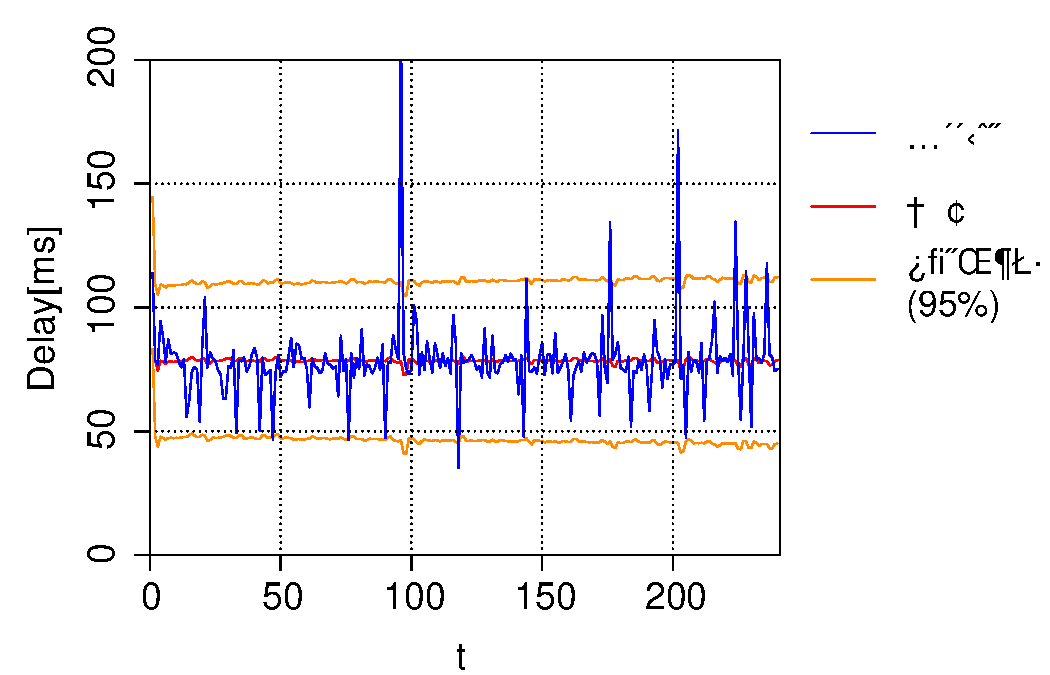
\includegraphics[width=7.5cm]{0302_07-plot.pdf}
}\\
\subfigure[3/9(月)7:00-8:00]{
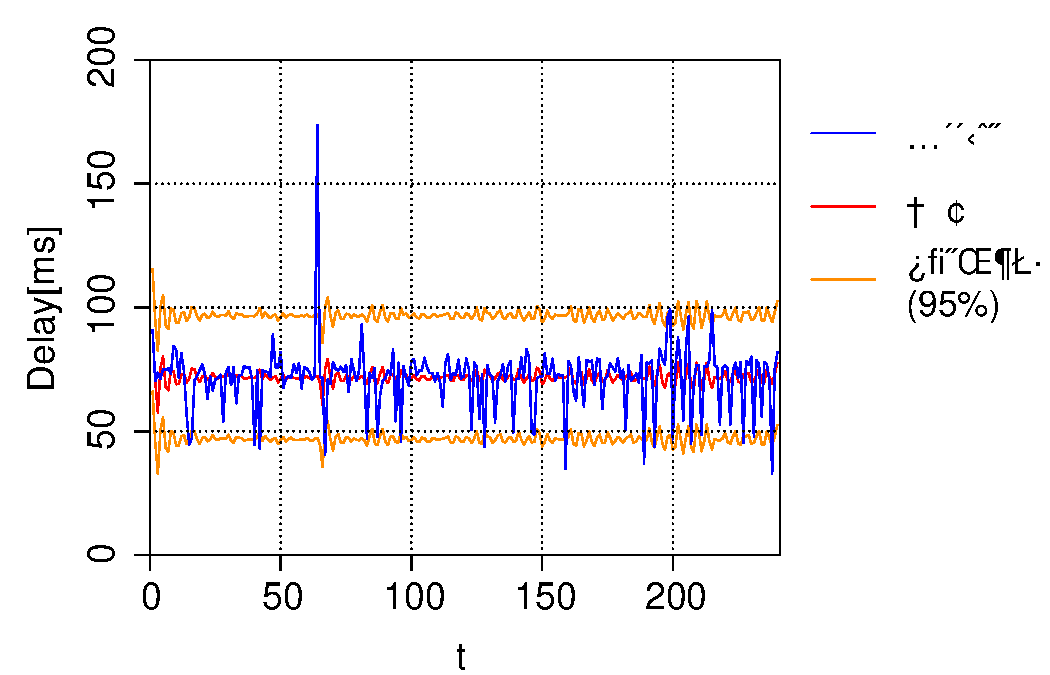
\includegraphics[width=7.5cm]{0309_07-plot.pdf}
}
\caption{月曜日の 7:00-8:00 計測の実測値に対する次数 (2,2,1,1) の ARMA-GARCH モデルによる回帰}
\label{norm-reg}
\end{center}
\end{figure}

\begin{figure}[tb]
\begin{center}
\subfigure[3/2(月)7:00-8:00]{
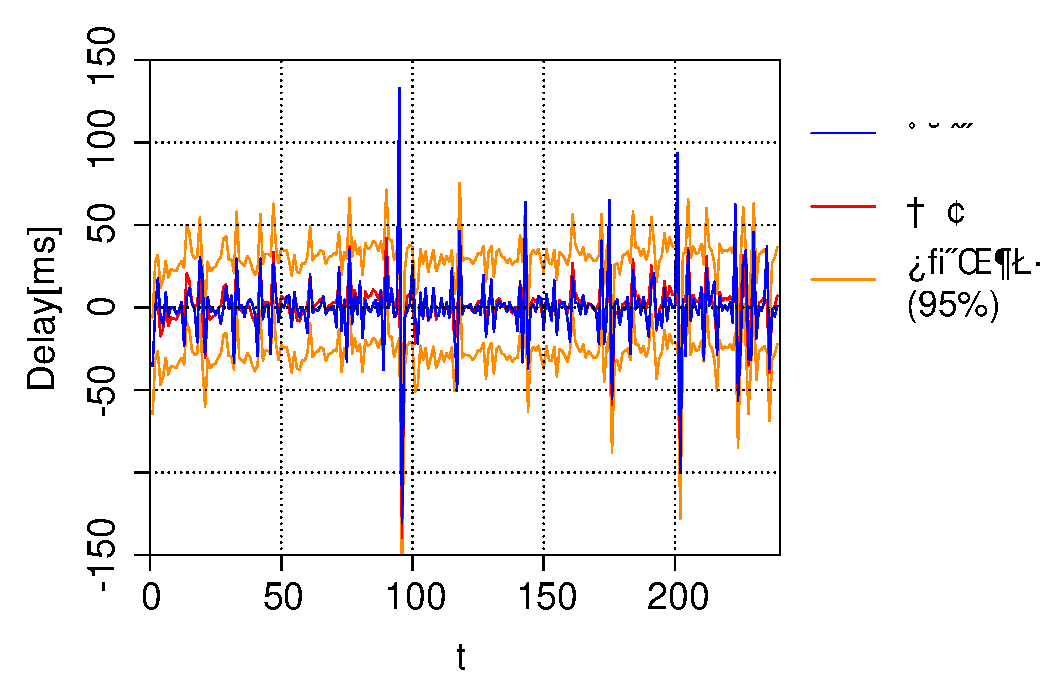
\includegraphics[width=7.5cm]{0302_07-plot-diff.pdf}
}\\
\subfigure[3/9(月)7:00-8:00]{
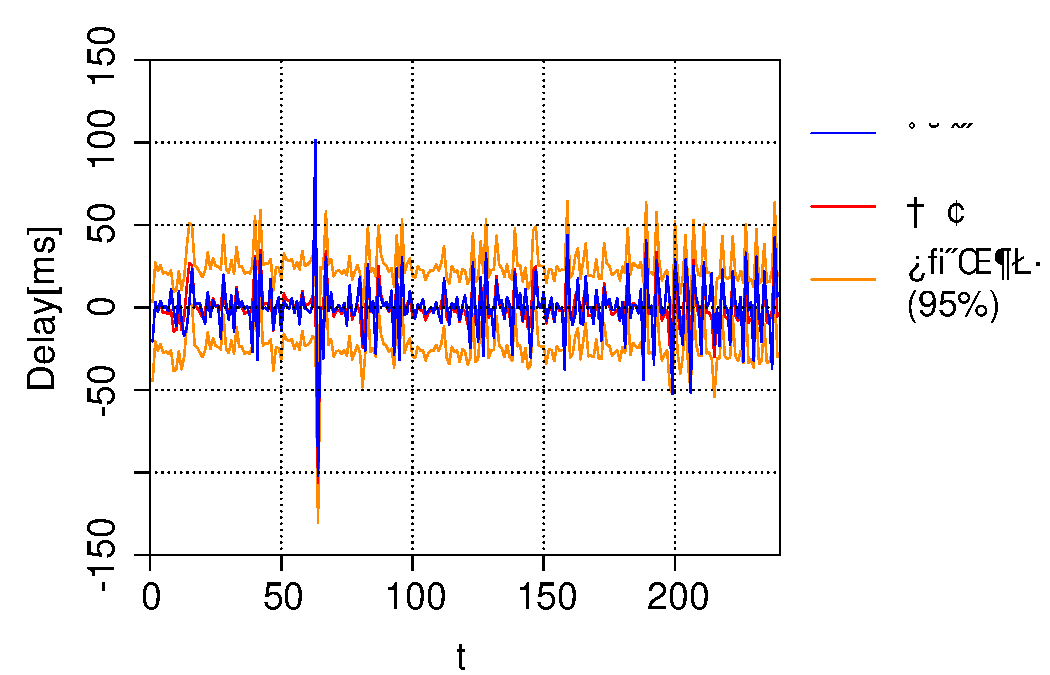
\includegraphics[width=7.5cm]{0309_07-plot-diff.pdf}
}
\caption{月曜日の 7:00-8:00 計測の変動値に対する次数 (2,2,1,1) の ARMA-GARCH モデルによる回帰}
\label{diff-reg}
\end{center}
\end{figure}

図 \ref{norm-reg} より,赤線で示される ARMA-GARCH モデルによる回帰線は青線で示された ping 応答の実測値の推移の傾向を大まかに捉えられている.
したがって,応答遅延時間が時間とともに単調に増加するなどの異常は,例えば工場内部の無線端末上でリアルタイムに ARMA-GARCH モデルによる応答遅延データの回帰を行うことで断続的に定まるパラメータの変化や,現場環境における通常時の傾向を反映した ARMA-GARCH のパラメータを用いて行った予測値から実測値が大きく外れ続けた場合などをもとに,検知することが可能と考える.
しかしながら一方で,単発的に発生する大きな応答遅延を予測できていない.
これは,この単発的に発生する応答遅延に周期性や過去データからみられる兆候がなく,予測が困難であることを示唆している.
この単発的な応答遅延によって,モデルの回帰精度が悪化したり,その発生頻度などに関する異常を検知できなかったりすることが考えられ,実用的な異常検知にむけてはこれらの点を改善するような別の手法と組み合わせることが必要だと思われる.
また,図 \ref{diff-reg} においては図 \ref{norm-reg} の場合と同様に,回帰線が変動値の推移をおおよそ捉えられ単発的な変動は捉えられていなかったものの,大きな ping 応答に対する立下りは捉えられていた.
このことから,変動値に対する ARMA-GARCH モデルではこれらの大きな応答遅延の単発性を表現できていると考えられる.
従って,大きな応答遅延が連続して発生するような異常は ARMA-GARCH モデルを用いることで検知可能ではないかと考えられる.

\begin{center}
Raspberry Pi の動作不良のため未使用の計測データ\\
3/6(金)17:00-18:00,3/7(土)17:00-18:00\\
3/12(木)12:00-13:00,3/12(木)17:00-18:00\\
3/13(金)17:00-18:00,3/14(土)17:00-18:00\\
3/15(日)17:00-18:00,3/16(月)17:00-18:00\\
3/17(火)20:00-21:00,3/20(金)17:00-18:00\\
3/22(日)17:00-18:00,3/23(月)12:00-13:00\\
3/23(月)20:00-21:00,3/24(火)17:00-18:00\\
3/24(火)20:00-21:00,3/25(水)20:00-21:00\\
3/26(木)20:00-21:00,3/27(金)20:00-21:00\\
\end{center}
\section{クラスタリングによる分類}
 ARMA-GARCH モデルを実測値データもしくは変動値データに対して適用した結果定まるパラメータ $W$ をもとにクラスタリングを行い,時間帯や場所ごとの ping 応答遅延特性を分析する.
また, $W$ は,実測値データと差分系列データともに
$$W = [c, a_1, a_2, b_1, b_2, \omega, \alpha_1, \beta_1] $$
で与えられる.


\bibliography{myrefs}
\bibliographystyle{sieicej}
\end{document}